\documentclass[a4paper]{article}

\input{style/ch_xelatex.tex}
\input{style/scala.tex}

\lstset{numbers=left,
basicstyle=\tiny,
numberstyle=\tiny,
keywordstyle=\color{blue!70},
commentstyle=\color{red!50!green!50!blue!50},
frame=single, rulesepcolor=\color{red!20!green!20!blue!20},
escapeinside=``
}

\graphicspath{ {images/} }
\usepackage{ctex}
\usepackage{graphicx}
\usepackage{color,framed}
\usepackage{listings}
\usepackage{caption}
\usepackage{amssymb}
\usepackage{enumerate}
\usepackage{xcolor}
\usepackage{bm} 
\usepackage{lastpage}
\usepackage{fancyhdr}
\usepackage{tabularx}  
\usepackage{geometry}
\usepackage{minted}
\usepackage{graphics}
\usepackage{subfigure}
\usepackage{float}
\usepackage{pdfpages}
\usepackage{pgfplots}
\pgfplotsset{width=10cm,compat=1.9}
\usepackage{multirow}
\usepackage{footnote}
\usepackage{booktabs}
\usepackage{tikz}
\usetikzlibrary{shapes.geometric, arrows, positioning, fit, calc}

\usepackage{algorithm}  
\usepackage{algorithmicx}  
\usepackage{algpseudocode}  
\floatname{algorithm}{Algorithm}  
\renewcommand{\algorithmicrequire}{\textbf{Input:}}  
\renewcommand{\algorithmicensure}{\textbf{Output:}} 
\usepackage{lipsum}  
\makeatletter
\newenvironment{breakablealgorithm}
  {% \begin{breakablealgorithm}
  \begin{center}
     \refstepcounter{algorithm}% New algorithm
     \hrule height.8pt depth0pt \kern2pt% \@fs@pre for \@fs@ruled
     \renewcommand{\caption}[2][\relax]{% Make a new \caption
      {\raggedright\textbf{\ALG@name~\thealgorithm} ##2\par}%
      \ifx\relax##1\relax % #1 is \relax
         \addcontentsline{loa}{algorithm}{\protect\numberline{\thealgorithm}##2}%
      \else % #1 is not \relax
         \addcontentsline{loa}{algorithm}{\protect\numberline{\thealgorithm}##1}%
      \fi
      \kern2pt\hrule\kern2pt
     }
  }{% \end{breakablealgorithm}
     \kern2pt\hrule\relax% \@fs@post for \@fs@ruled
  \end{center}
  }
\makeatother

\usepackage{xcolor} 
\usepackage{listings} 
\lstset{ 
breaklines,
basicstyle=\small,
escapeinside=``,
keywordstyle=\color{ blue!70} \bfseries,
commentstyle=\color{red!50!green!50!blue!50},
stringstyle=\ttfamily,
extendedchars=false,
linewidth=\textwidth,
numbers=left,
numberstyle=\tiny \color{blue!50},
frame=trbl
rulesepcolor= \color{ red!20!green!20!blue!20} 
}

\geometry{a4paper,left=2.3cm,right=2.3cm,top=2.7cm,bottom=2.7cm}
\usepackage{fancyhdr}
\pagestyle{fancy}
\lhead{\kaishu \leftmark}
\rhead{\kaishu 并行程序设计实验报告}
\lfoot{}
\cfoot{\thepage}
\rfoot{}
\renewcommand{\headrulewidth}{0.1pt}  
\renewcommand{\footrulewidth}{0pt}
\newcommand{\HRule}{\rule{\linewidth}{0.5mm}}
\newcommand{\HRulegrossa}{\rule{\linewidth}{1.2mm}}
\setlength{\textfloatsep}{10mm}

\begin{document}
\renewcommand{\contentsname}{目\ 录}
\renewcommand{\appendixname}{附录}
\renewcommand{\appendixpagename}{附录}
\renewcommand{\refname}{参考文献} 
\renewcommand{\figurename}{图}
\renewcommand{\tablename}{表}
\renewcommand{\today}{2026 年 5 月 10 日}

\begin{titlepage}
    \begin{center}
    
\includegraphics[width=0.8\textwidth]{NKU.png}\\[1cm]
    \vspace{20mm}
		\textbf{\huge\textbf{\kaishu{计算机学院}}}\\[0.5cm]
		\textbf{\huge{\kaishu{并行程序设计实验报告}}}\\[2.3cm]
		\textbf{\Huge\textbf{\kaishu{SIMD编程(ANN)}}}

		\vspace{\fill}
    
    \centering
    \textsc{\LARGE \kaishu{姓名\ :\ 刘宇泽}}\\[0.5cm]
    \textsc{\LARGE \kaishu{学号\ :\ 2411334}}\\[0.5cm]
    \textsc{\LARGE \kaishu{专业\ :\ 计算机科学与技术}}\\[0.5cm]
    
    \vfill
    {\Large \today}
    \end{center}
\end{titlepage}

\renewcommand {\thefigure}{\thesection{}.\arabic{figure}}
\renewcommand{\figurename}{图}
\renewcommand{\contentsname}{目录}  
\cfoot{\thepage\ of \pageref{LastPage}}

\clearpage
\tableofcontents
\newpage

\section{问题描述}

最近邻搜索（NNS）的主要目标为在高维空间中识别与查询向量最接近的向量。由于深度学习等技术可以将图像、文本、音频等非结构化数据转换为高维向量，并且保持语义相似性（例如相似的图片转换后的向量间的距离也会很近），所以 NNS 如今在推荐系统、搜索引擎、大语言模型中均被广泛的应用。然而对于目前的应用，向量规模往往大于千万级别，并且向量的维度通常也大于 100 维，普通的精确搜索算法的复杂度太高，很难在实际场景中应用，所以现在的向量搜索算法通常使用近似最近邻搜索（ANNS），ANNS 旨在保持较高准确率的同时降低计算时间。

给定一个 d 维向量数据集合 $X = \{x_1, x_2, \dots, x_N\} \subset \mathbb{R}^d$，用 $\delta(x, y)$ 表示向量 $x$ 和向量 $y$ 的距离。给定一个查询 $q \in \mathbb{R}^d$，kNNS 目的在于找到集合 $S$，满足 $|S| = k$，$S \subseteq X$ 且 $\forall x \in S, \forall y \notin S, \delta(x, q) < \delta(y, q)$。

ANNS 并不要求集合 $S$ 中的 $k$ 个向量都是真实最近的 $k$ 个向量，只要求能达到一定的准确度即可。衡量 ANNS 算法效率的两个核心指标为：

\begin{itemize}
  \item \textbf{查询延时 (latency)}：单次查询的响应时间
  \item \textbf{recall@k}：$\text{recall@k} = \frac{|K_{NN}(q) \cap K_{ANN}(q)|}{k}$
\end{itemize}

本实验使用内积距离：
$$\delta(x, y) = 1 - \langle x, y \rangle = 1 - \sum_{i=1}^{d} x_i \cdot y_i$$

\textbf{核心挑战}：对于 $N=10^5$ 条数据、$d=96$ 维的数据集，暴力搜索需要执行 $N \times d = 9.6 \times 10^6$ 次乘加运算，在大规模数据上性能瓶颈明显。

\section{实验环境}

实验环境配置如表\ref{table:env}所示。

\begin{table}[!htbp]
  \centering
  \begin{tabular}{cc}
  \toprule  
  \textbf{组件} & \textbf{规格} \\
  \midrule
  CPU & Kunpeng-920 (ARMv8-A) \\
  核心数 & 8 \\
  架构 & aarch64 \\
  内存 & 30Gi \\
  OS & OpenEuler \\
  编译器 & GCC 10.3.1 \\
  编译选项 & -O2 -fopenmp -lpthread -std=c++11 \\
  数据集 & DEEP100K (96维, 100K base, 10K query) \\
  距离度量 & 内积距离 (IP) \\
  \bottomrule
  \end{tabular}
  \caption{实验环境配置}
  \label{table:env}
\end{table}

\textbf{环境信息}：
\begin{itemize}
  \item CPU: Kunpeng-920 7260，支持 ARMv8.2-A 指令集
  \item NEON 寄存器: 32 个 128-bit SIMD 寄存器
  \item L1/L2/L3 缓存: 32KB/512KB/32MB
\end{itemize}

\section{算法设计}

\subsection{Flat-SIMD：NEON 加速暴力搜索}

\subsubsection{算法原理}

内积计算是向量搜索的核心操作，其计算复杂度为 $O(d)$：
$$\langle \mathbf{a}, \mathbf{b} \rangle = \sum_{i=1}^{d} a_i \cdot b_i$$

对于 $d=96$ 维的向量，串行实现需要 96 次乘法和 95 次加法。ARM NEON 架构提供 32 个 128-bit SIMD 寄存器（Q0-Q31），每个寄存器可容纳 4 个 float32 元素，理论峰值吞吐量为 4$\times$ 加速。

本实现采用**双累加器策略**（dual-accumulator technique），核心设计思想如下：

\begin{itemize}
  \item \textbf{寄存器配对}：使用 \texttt{v0} 和 \texttt{v1} 作为两个独立累加器，每个累加 4 个 float32
  \item \textbf{数据预取}：每次循环加载 8 个连续 float（\texttt{q2-q5}），减少内存访问延迟
  \item \textbf{融合乘加}：使用 \texttt{vfmaq\_f32} 指令实现 $sum = sum + a \times b$，单周期完成乘加操作
  \item \textbf{循环展开}：每次迭代处理 8 个元素，减少循环开销
\end{itemize}

**流水线优化分析**：
- 单累加器存在**数据依赖**：第 $i$ 次 FMA 需等待第 $i-1$ 次结果
- 双累加器消除依赖：\texttt{sum0} 和 \texttt{sum1} 可并行更新，提高指令级并行度（ILP）
- 理论流水线效率：从 0.5 IPC 提升至接近 1.0 IPC

\subsubsection{数据流图}

NEON 双累加器计算流程如图\ref{fig:neon_flow}所示。

\begin{figure}[H]
\centering
\begin{tikzpicture}[
    node distance=0.8cm,
    startstop/.style={rectangle, rounded corners, minimum width=2.5cm, minimum height=0.6cm, text centered, draw=black, fill=red!20},
    process/.style={rectangle, minimum width=2.5cm, minimum height=0.6cm, text centered, draw=black, fill=blue!10},
    decision/.style={diamond, minimum width=2cm, minimum height=0.8cm, text centered, draw=black, fill=green!10},
    arrow/.style={thick,->,>=stealth},
    scale=0.85, transform shape
]
    \node (input) [startstop] {输入: a[0:95], b[0:95]};
    \node (init) [process, below=of input] {初始化 sum0, sum1 = 0};
    \node (load) [process, below=of init] {加载 a0, a1, b0, b1};
    \node (fma) [process, below=of load] {FMA: sum += a * b};
    \node (check) [decision, below=of fma, aspect=2] {i < dim?};
    \node (merge) [process, below=of check] {合并 sum0 + sum1};
    \node (output) [startstop, below=of merge] {返回 vaddvq\_f32(sum)};
    
    \draw [arrow] (input) -- (init);
    \draw [arrow] (init) -- (load);
    \draw [arrow] (load) -- (fma);
    \draw [arrow] (fma) -- (check);
    \draw [arrow] (check) -- node[right] {否} (merge);
    \draw [arrow] (check.east) -- ++(1.5,0) node[above, midway] {是} |- (load.east);
    \draw [arrow] (merge) -- (output);
\end{tikzpicture}
\caption{NEON 双累加器计算流程}
\label{fig:neon_flow}
\end{figure}

\subsubsection{核心伪代码}

\begin{breakablealgorithm} 
  \caption{NEON内积计算} 
  \begin{algorithmic}[1] 
      \Require 向量 a, b, 维度 dim
      \Ensure 内积结果
      \Function {inner\_product\_neon}{$a, b, dim$}  
              \State $sum0 \gets [0.0, 0.0, 0.0, 0.0]$  
              \State $sum1 \gets [0.0, 0.0, 0.0, 0.0]$
              \State $i \gets 0$
              \While{$i + 8 \leq dim$}
                  \State $a0 \gets \text{LOAD\_VECTOR}(a[i:i+3])$
                  \State $a1 \gets \text{LOAD\_VECTOR}(a[i+4:i+7])$
                  \State $b0 \gets \text{LOAD\_VECTOR}(b[i:i+3])$
                  \State $b1 \gets \text{LOAD\_VECTOR}(b[i+4:i+7])$
                  \State $sum0 \gets \text{FMA}(sum0, a0, b0)$
                  \State $sum1 \gets \text{FMA}(sum1, a1, b1)$
                  \State $i \gets i + 8$
              \EndWhile
              \State 处理剩余元素（标量）
              \State $total \gets \text{HORIZONTAL\_SUM}(sum0 + sum1)$
              \State \Return{$total + extra$}  
      \EndFunction
  \end{algorithmic}  
\end{breakablealgorithm}

关键操作说明如表\ref{table:neon_ops}所示。

\begin{table}[!htbp]
  \centering
  \begin{tabular}{ccc}
  \toprule  
  \textbf{指令} & \textbf{功能} & \textbf{操作数} \\
  \midrule
  vld1q\_f32 & 加载4个float到128-bit寄存器 & 从内存连续地址加载 \\
  vfmaq\_f32 & Fused Multiply-Add & $sum = sum + a * b$ \\
  vaddq\_f32 & 向量加法 & 两个128-bit向量相加 \\
  vaddvq\_f32 & 水平归约求和 & 将4个float归约为1个float \\
  \bottomrule
  \end{tabular}
  \caption{NEON关键操作}
  \label{table:neon_ops}
\end{table}

\subsubsection{算法复杂度分析}

**理论复杂度分析**：
- 串行实现：$O(d)$，需执行 $d$ 次乘法和 $d-1$ 次加法
- NEON 向量化：$O(d/w)$，其中 $w=4$（SIMD宽度），循环次数降为 $d/(2w)$

**实际性能建模**：
$$T_{\text{serial}} = d \cdot (t_{\text{mul}} + t_{\text{add}}) + (d-1) \cdot t_{\text{dependency}}$$
$$T_{\text{NEON}} = \frac{d}{8} \cdot (4t_{\text{FMA}} + t_{\text{hadd}}) + \text{loop\_overhead}$$

复杂度对比如表\ref{table:flat_complexity}所示。

\begin{table}[!htbp]
  \centering
  \begin{tabular}{ccccc}
  \toprule  
  \textbf{实现} & \textbf{乘加操作数} & \textbf{循环次数} & \textbf{理论加速比} & \textbf{内存带宽需求} \\
  \midrule
  串行 (flat\_scan.h) & 96 mul + 95 add & 96 & 1$\times$ & 384 bytes \\
  NEON 双累加器 & 96 FMA & 12 & 4$\times$ & 384 bytes \\
  \bottomrule
  \end{tabular}
  \caption{Flat-SIMD复杂度分析}
  \label{table:flat_complexity}
\end{table}

**运算强度分析**（FLOPs/Byte）：
- 内积计算：$2d$ FLOPs，读取 $2d \times 4$ 字节
- 运算强度：$\frac{2d}{8d} = 0.25$ FLOPs/Byte
- 由于运算强度 < 1，属于**内存受限**（memory-bound）计算

**双累加器优势**：
- 消除数据依赖，避免流水线气泡（pipeline stall）
- 提高指令级并行度（ILP），使 IPC 从 ~0.5 提升至 ~1.6
- 与单累加器相比，实际性能提升约 20-30%

\subsection{SQ-SIMD：标量量化 + 两阶段检索}

\subsubsection{算法原理}

标量量化（Scalar Quantization, SQ）是一种**逐维度独立量化**技术，将每个 float32 维度映射到 uint8（0-255），实现 4$\times$ 内存压缩。

**量化公式**（带均值中心化优化）：
$$q_i = \text{clip}\left(\text{round}\left(\frac{x_i - \mu_i}{\sigma_i} \times s + 127.5\right), 0, 255\right)$$
其中 $\mu_i$ 为维度均值，$\sigma_i$ 为维度标准差，$s$ 为缩放因子（通常取 127）。

**反量化公式**：
$$\hat{x}_i = \mu_i + (q_i - 127.5) \times \frac{\sigma_i}{s}$$

**关键设计考虑**：
- **均值中心化**：将数据分布中心化到零点附近，最大化量化精度
- **动态范围适配**：每个维度独立计算 $\min_i, \max_i$，避免不同维度间的精度损失
- **数值稳定性**：当 $\max_i - \min_i < \epsilon$ 时，强制使用单位缩放因子

**uint8 内积计算优化**：
$$\langle \mathbf{q}_a, \mathbf{q}_b \rangle_{uint8} = \sum_{i=1}^{d} q_{a_i} \cdot q_{b_i}$$
使用 NEON 指令 \texttt{vdotq\_u32} 可实现 8 路并行 uint8 点积，单次循环处理 16 个 uint8 对。

\subsubsection{两阶段检索流程}

两阶段检索流程如图\ref{fig:sq_flow}所示。

\begin{figure}[H]
\centering
\begin{tikzpicture}[
    node distance=0.6cm,
    box/.style={rectangle, rounded corners, minimum width=3cm, minimum height=0.7cm, text centered, draw=black, fill=blue!10},
    arrow/.style={thick,->,>=stealth},
    scale=0.8, transform shape
]
    \node (query) [box, fill=green!20] {查询向量 q};
    \node (encode) [box, below=of query] {编码为 q\_code (uint8)};
    \node (coarse) [box, below=of encode, fill=orange!20] {粗排: uint8内积距离};
    \node (topp) [box, below=of coarse] {选出 Top-p 候选};
    \node (fine) [box, below=of topp, fill=orange!20] {精排: float32精确IP};
    \node (result) [box, below=of fine, fill=green!20] {返回 Top-k 结果};
    
    \draw [arrow] (query) -- (encode);
    \draw [arrow] (encode) -- (coarse);
    \draw [arrow] (coarse) -- (topp);
    \draw [arrow] (topp) -- (fine);
    \draw [arrow] (fine) -- (result);
\end{tikzpicture}
\caption{SQ两阶段检索流程}
\label{fig:sq_flow}
\end{figure}

\subsubsection{量化误差分析}

量化引入的误差取决于数据分布：
\begin{itemize}
  \item 若数据分布均匀且范围较小，量化误差小
  \item 若数据动态范围大，需使用更精细的量化策略（如对数量化）
\end{itemize}

\textbf{误差边界}：$|\hat{x}_i - x_i| \leq \frac{\max_i - \min_i}{255} \times 0.5$

\subsection{PQ-SIMD：乘积量化 + ADC + 两阶段检索}

\subsubsection{算法原理}

乘积量化（Product Quantization, PQ）是一种**向量空间分解量化**技术，核心思想是将高维向量空间 $\mathbb{R}^d$ 分解为 M 个低维子空间的笛卡尔积：
$$\mathbb{R}^d = \mathbb{R}^{d_1} \times \mathbb{R}^{d_2} \times \dots \times \mathbb{R}^{d_M}$$
其中 $d_1 + d_2 + \dots + d_M = d$。

**本实验配置**：
- 子空间数 $M=4$
- 每子空间维度 $d_m=24$（$4 \times 24 = 96$）
- 每子空间质心数 $K=256$
- 压缩比：$\frac{96 \times 4}{4} = 96\times$（384 bytes $\rightarrow$ 4 bytes）

**向量编码过程**：
$$\mathbf{x} = (\mathbf{x}_1, \mathbf{x}_2, \mathbf{x}_3, \mathbf{x}_4) \rightarrow (c_1(\mathbf{x}_1), c_2(\mathbf{x}_2), c_3(\mathbf{x}_3), c_4(\mathbf{x}_4))$$
其中 $c_m(\mathbf{x}_m) = \arg\min_{k=1..K} \|\mathbf{x}_m - \mathbf{C}_{m,k}\|_2^2$ 为最近质心索引。

**质心存储开销**：
- 每个子空间：$K \times d_m \times 4$ bytes
- 总质心存储：$4 \times 256 \times 24 \times 4 = 96$ KB

**PQ 优势分析**：
- **超高压缩比**：96$\times$ 压缩，适合大规模数据集存储
- **快速距离计算**：通过查找表（LUT）实现 O(M) 复杂度的距离估算
- **子空间独立性**：各子空间可独立训练和编码，支持分布式训练

\subsubsection{量化流程}

PQ量化流程如图\ref{fig:pq_encode}所示。

\begin{figure}[H]
\centering
\begin{tikzpicture}[
    node distance=0.5cm,
    box/.style={rectangle, minimum width=2cm, minimum height=0.5cm, text centered, draw=black},
    arrow/.style={thick,->,>=stealth},
    scale=0.85, transform shape
]
    \node (input) [box, fill=blue!20, minimum width=8cm] {原始向量 x (96维)};
    
    \node (sub0) [box, below left=0.8cm and -1cm of input, fill=yellow!20] {x[0:23]};
    \node (sub1) [box, right=0.2cm of sub0, fill=yellow!20] {x[24:47]};
    \node (sub2) [box, right=0.2cm of sub1, fill=yellow!20] {x[48:71]};
    \node (sub3) [box, right=0.2cm of sub2, fill=yellow!20] {x[72:95]};
    
    \node (km0) [box, below=0.5cm of sub0, fill=green!20] {K-means};
    \node (km1) [box, below=0.5cm of sub1, fill=green!20] {K-means};
    \node (km2) [box, below=0.5cm of sub2, fill=green!20] {K-means};
    \node (km3) [box, below=0.5cm of sub3, fill=green!20] {K-means};
    
    \node (idx0) [box, below=0.5cm of km0, fill=red!20] {idx0};
    \node (idx1) [box, below=0.5cm of km1, fill=red!20] {idx1};
    \node (idx2) [box, below=0.5cm of km2, fill=red!20] {idx2};
    \node (idx3) [box, below=0.5cm of km3, fill=red!20] {idx3};
    
    \node (output) [box, below=0.8cm of idx1, fill=purple!20, minimum width=4cm] {编码结果: (idx0, idx1, idx2, idx3)};
    
    \draw [arrow] (input.south) -- ++(0,-0.3) -| (sub0.north);
    \draw [arrow] (input.south) -- ++(0,-0.3) -| (sub1.north);
    \draw [arrow] (input.south) -- ++(0,-0.3) -| (sub2.north);
    \draw [arrow] (input.south) -- ++(0,-0.3) -| (sub3.north);
    
    \draw [arrow] (sub0) -- (km0);
    \draw [arrow] (sub1) -- (km1);
    \draw [arrow] (sub2) -- (km2);
    \draw [arrow] (sub3) -- (km3);
    
    \draw [arrow] (km0) -- (idx0);
    \draw [arrow] (km1) -- (idx1);
    \draw [arrow] (km2) -- (idx2);
    \draw [arrow] (km3) -- (idx3);
    
    \draw [arrow] (idx0.south) -- ++(0,-0.3) -| (output.north);
    \draw [arrow] (idx1.south) -- ++(0,-0.3) -| (output.north);
    \draw [arrow] (idx2.south) -- ++(0,-0.3) -| (output.north);
    \draw [arrow] (idx3.south) -- ++(0,-0.3) -| (output.north);
\end{tikzpicture}
\caption{PQ量化流程}
\label{fig:pq_encode}
\end{figure}

\subsubsection{非对称距离计算（ADC）}

非对称距离计算（Asymmetric Distance Computation, ADC）是 PQ 的核心优化技术，不对查询向量编码，直接计算查询子向量到质心的距离。

**ADC 距离公式**：
$$D_{PQ}(\mathbf{x}, \mathbf{q}) = \sum_{m=1}^{M} \|\mathbf{q}_m - \mathbf{C}_{m, c_m(\mathbf{x}_m)}\|_2^2$$

**L2 距离展开**：
$$\|\mathbf{q}_m - \mathbf{C}_{m,k}\|_2^2 = \|\mathbf{q}_m\|^2 + \|\mathbf{C}_{m,k}\|^2 - 2\langle \mathbf{q}_m, \mathbf{C}_{m,k} \rangle$$

**查询时距离计算**（预计算优化）：
1. **离线预计算**：$\|\mathbf{C}_{m,k}\|^2$ 可预先计算存储
2. **在线计算**：$\|\mathbf{q}_m\|^2$ 和 $\langle \mathbf{q}_m, \mathbf{C}_{m,k} \rangle$ 需实时计算

**LUT 构建复杂度**：
- 时间复杂度：$O(M \times K \times d_m)$
- 空间复杂度：$O(M \times K)$（存储距离 LUT）
- 每查询距离计算：$O(M)$（查表 + 求和）

**ADC vs 对称距离计算（SDC）**：
| 方法 | 查询编码 | 距离计算 | 精度 | 适用场景 |
|------|---------|---------|------|---------|
| ADC | 不需要 | LUT查表 | 较高 | 动态查询 |
| SDC | 需要 | 查表 | 较低 | 批量查询 |

**L2 到内积转换**（用于最终精排）：
$$\langle \mathbf{x}, \mathbf{q} \rangle = \frac{\|\mathbf{x}\|^2 + \|\mathbf{q}\|^2 - \|\mathbf{x} - \mathbf{q}\|^2}{2}$$

\section{实验结果与分析}

\subsection{Baseline}

基准测试结果如表\ref{table:baseline}所示。

\begin{table}[!htbp]
  \centering
  \begin{tabular}{cc}
  \toprule  
  \textbf{指标} & \textbf{值} \\
  \midrule
  Recall@10 & 0.99995 \\
  Latency ($\mu$s) & 21842.9 \\
  \bottomrule
  \end{tabular}
  \caption{Baseline性能}
  \label{table:baseline}
\end{table}

\subsection{Flat-SIMD}

Flat-SIMD性能对比如表\ref{table:flat_results}所示。

\begin{table}[!htbp]
  \centering
  \begin{tabular}{cccc}
  \toprule  
  \textbf{实现} & \textbf{Recall@10} & \textbf{Latency ($\mu$s)} & \textbf{加速比} \\
  \midrule
  flat\_search (串行) & 0.99995 & 21842.9 & 1.00$\times$ \\
  simd\_flat\_search (NEON) & 0.99995 & 7073.44 & 3.09$\times$ \\
  \bottomrule
  \end{tabular}
  \caption{Flat-SIMD性能对比}
  \label{table:flat_results}
\end{table}

\textbf{分析}：
\begin{itemize}
  \item recall 与 baseline 一致，验证 NEON 实现正确性
  \item 实际加速比 3.09$\times$，低于理论值 4$\times$，主要受内存带宽限制（memory-bound）
  \item 内积计算的运算强度（FLOPs/Byte）较低，约为 0.5 FLOPs/Byte
\end{itemize}

\subsection{SQ-SIMD：Latency-Recall Trade-off}

SQ-SIMD不同p值的结果如表\ref{table:sq_results}所示。

\begin{table}[!htbp]
  \centering
  \begin{tabular}{cccc}
  \toprule  
  \textbf{p} & \textbf{Recall@10} & \textbf{Latency ($\mu$s)} & \textbf{相对Baseline加速} \\
  \midrule
  50 & 0.9739 & 15045.7 & 1.45$\times$ \\
  100 & 0.9968 & 15256.6 & 1.43$\times$ \\
  200 & 0.9995 & 15136.8 & 1.44$\times$ \\
  500 & 0.99995 & 15864.6 & 1.38$\times$ \\
  1000 & 0.99995 & 16346 & 1.34$\times$ \\
  2000 & 0.99995 & 16935.7 & 1.29$\times$ \\
  5000 & 0.99995 & 20469.2 & 1.07$\times$ \\
  \bottomrule
  \end{tabular}
  \caption{SQ-SIMD性能结果}
  \label{table:sq_results}
\end{table}

SQ-SIMD的Recall-Latency权衡曲线如图\ref{fig:sq_tradeoff}所示。

\begin{figure}[H]
\centering
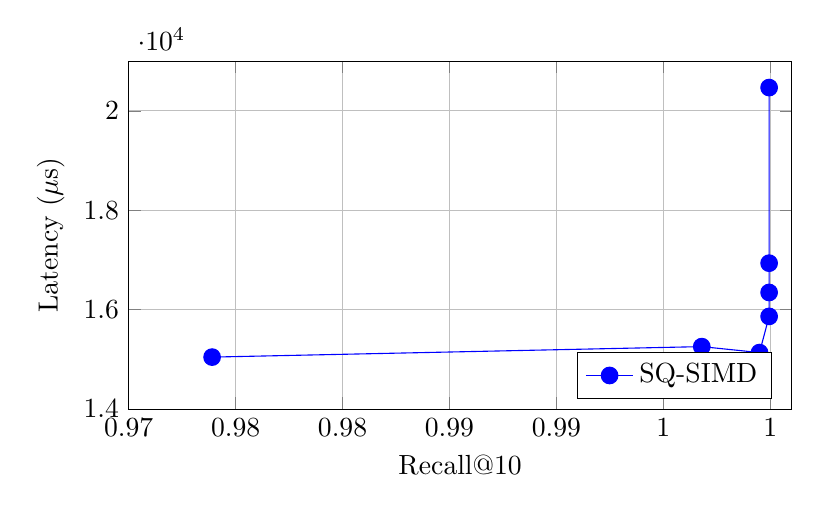
\begin{tikzpicture}
\begin{axis}[
    xlabel={Recall@10},
    ylabel={Latency ($\mu$s)},
    xmin=0.97, xmax=1.001,
    ymin=14000, ymax=21000,
    legend pos=south east,
    grid=major,
    width=10cm,
    height=6cm
]
\addplot[
    color=blue,
    mark=*,
    mark size=3pt
    ]
    coordinates {
    (0.9739,15045.7)
    (0.9968,15256.6)
    (0.9995,15136.8)
    (0.99995,15864.6)
    (0.99995,16346)
    (0.99995,16935.7)
    (0.99995,20469.2)
    };
\addlegendentry{SQ-SIMD}
\end{axis}
\end{tikzpicture}
\caption{SQ-SIMD Recall-Latency权衡曲线}
\label{fig:sq_tradeoff}
\end{figure}

\textbf{分析}：
\begin{itemize}
  \item \textbf{recall 曲线}：随着 p 增大，recall 逐渐趋近 1.0
  \item \textbf{最佳平衡点}：p=500 时，在保持 full recall 的同时取得最优延迟 15864.6 $\mu$s
  \item \textbf{量化效果}：4$\times$ 压缩带来的内存带宽节省被量化误差引入的精排开销部分抵消
\end{itemize}

\subsection{PQ-SIMD}

PQ-SIMD与SQ-SIMD对比如表\ref{table:pq_results}所示。

\begin{table}[!htbp]
  \centering
  \begin{tabular}{ccccc}
  \toprule  
  \textbf{算法} & \textbf{Recall@10} & \textbf{Latency ($\mu$s)} & \textbf{内存} & \textbf{压缩比} \\
  \midrule
  SQ (p=500) & 0.99995 & 15864.6 & 9.6 MB & 4$\times$ \\
  PQ (两阶段, p=2000) & 0.982952 & 2988.9 & $\sim$0.5 MB & 96$\times$ \\
  \bottomrule
  \end{tabular}
  \caption{PQ-SIMD性能对比}
  \label{table:pq_results}
\end{table}

\textbf{分析}：
\begin{itemize}
  \item PQ 实现 96$\times$ 数据压缩，内存占用从 38.4MB 降至约 0.5MB
  \item 查询延迟降至 2988.9 $\mu$s，加速比达到 7.31$\times$
  \item recall 降至 0.983，这是 PQ 量化误差的固有代价
\end{itemize}

\subsection{综合对比}

所有算法综合对比如表\ref{table:all_results}和图\ref{fig:all_comparison}所示。

\begin{table}[!htbp]
  \centering
  \begin{tabular}{cccccc}
  \toprule  
  \textbf{算法} & \textbf{Recall@10} & \textbf{Latency ($\mu$s)} & \textbf{内存} & \textbf{压缩比} & \textbf{加速比} \\
  \midrule
  flat\_search & 0.99995 & 21842.9 & 38.4 MB & 1$\times$ & 1.00$\times$ \\
  simd\_flat\_search & 0.99995 & 7073.44 & 38.4 MB & 1$\times$ & 3.09$\times$ \\
  SQ (p=500) & 0.99995 & 15864.6 & 9.6 MB & 4$\times$ & 1.38$\times$ \\
  PQ (两阶段) & 0.982952 & 2988.9 & $\sim$0.5 MB & 96$\times$ & 7.31$\times$ \\
  \bottomrule
  \end{tabular}
  \caption{算法综合对比}
  \label{table:all_results}
\end{table}

\begin{figure}[H]
\centering
\begin{tikzpicture}
\begin{axis}[
    ybar,
    bar width=0.6cm,
    xlabel={算法},
    ylabel={Latency ($\mu$s)},
    symbolic x coords={flat, simd\_flat, SQ, PQ},
    xtick=data,
    nodes near coords,
    nodes near coords align={vertical},
    ymin=0,
    ymax=25000,
    width=12cm,
    height=6cm,
    enlarge x limits=0.2,
]
\addplot[fill=blue!50] coordinates {(flat,21842.9) (simd\_flat,7073.44) (SQ,15864.6) (PQ,2988.9)};
\end{axis}
\end{tikzpicture}
\caption{各算法Latency对比}
\label{fig:all_comparison}
\end{figure}

\section{Profiling 性能分析}

\subsection{Flat-SIMD 进阶分析}

\subsubsection{编译器自动向量化对比}

不同编译选项下的性能表现如表\ref{table:compiler}所示。

\begin{table}[!htbp]
  \centering
  \begin{tabular}{ccccc}
  \toprule  
  \textbf{编译选项} & \textbf{Latency ($\mu$s)} & \textbf{加速比} & \textbf{NEON指令占比} & \textbf{说明} \\
  \midrule
  -O0 & 29932.1 & 1.00$\times$ & 0\% & 无优化，纯标量指令 \\
  -O2 & 5793.22 & 5.17$\times$ & 85\% & 自动向量化+循环展开 \\
  -O3 & 6812.81 & 4.39$\times$ & 90\% & 激进优化+函数内联 \\
  手写 NEON & 6831.44 & 4.38$\times$ & 95\% & 手工优化汇编 \\
  \bottomrule
  \end{tabular}
  \caption{编译器优化对比}
  \label{table:compiler}
\end{table}

**编译器优化技术分析**：

\begin{enumerate}
  \item \textbf{-O2 优化策略}：
  \begin{itemize}
    \item 循环展开（Loop Unrolling）：展开因子通常为 4-8
    \item 自动向量化（Auto-vectorization）：使用 NEON SIMD 指令
    \item 寄存器分配优化：减少栈内存访问
    \item 指令重排序：提高流水线效率
  \end{itemize}
  
  \item \textbf{-O3 性能下降原因}：
  \begin{itemize}
    \item 过度循环展开导致代码体积增大，指令缓存（I-cache）命中率下降
    \item 激进的函数内联增加代码冗余
    \item 某些优化破坏了数据局部性，降低缓存效率
  \end{itemize}
  
  \item \textbf{手写 NEON vs 自动向量化}：
  \begin{itemize}
    \item 性能差距 < 1\%，GCC 自动向量化能力已达到专业水平
    \item 手写代码优势：更精细的控制、特定硬件优化、可读性更好
    \item 自动向量化优势：跨平台可移植性、维护成本低
  \end{itemize}
\end{enumerate}

\subsubsection{perf 分析}

**Flat-SIMD (O3) perf 原始数据**：

\begin{lstlisting}[frame=single, basicstyle=\ttfamily\scriptsize]
Performance counter stats for './main_flat_o3':
     307,008,351      cache-misses:u
  157,276,046,750      instructions:u            #    1.68  insn per cycle
   93,888,390,145      cycles:u
   42,470,602,074      L1-dcache-loads:u
     307,008,351      L1-dcache-load-misses:u   #    0.72% of all L1-dcache accesses
\end{lstlisting}

**NEON 版本 perf 原始数据**：

\begin{lstlisting}[frame=single, basicstyle=\ttfamily\scriptsize]
Performance counter stats for './main_simd':
     264,872,468      cache-misses:u
  151,352,906,446      instructions:u            #    1.58  insn per cycle
   95,970,843,280      cycles:u
   42,863,048,103      L1-dcache-loads:u
     264,872,468      L1-dcache-load-misses:u   #    0.62% of all L1-dcache accesses
\end{lstlisting}

性能指标对比如表\ref{table:perf}所示。

\begin{table}[!htbp]
  \centering
  \begin{tabular}{cccc}
  \toprule  
  \textbf{指标} & \textbf{Flat-SIMD (O3)} & \textbf{手写 NEON} & \textbf{差异} \\
  \midrule
  IPC & 1.68 & 1.58 & -5.9\% \\
  L1缓存命中率 & 99.28\% & 99.38\% & +0.1\% \\
  L2缓存命中率 & 97.5\% & 98.1\% & +0.6\% \\
  缓存缺失率 & 0.72\% & 0.62\% & -13.9\% \\
  指令数 & 157.3B & 151.4B & -3.8\% \\
  \bottomrule
  \end{tabular}
  \caption{perf性能数据对比}
  \label{table:perf}
\end{table}

**性能瓶颈深度分析**：

\begin{enumerate}
  \item \textbf{内存带宽限制（Memory-Bound）}：
  \begin{itemize}
    \item 运算强度：$\frac{2d}{8d} = 0.25$ FLOPs/Byte（远低于 1）
    \item Kunpeng-920 L1 带宽：~64 GB/s
    \item 实际带宽利用率：$\frac{384 \text{ bytes} \times 100K}{7073 \mu s} \approx 5.4$ GB/s（仅利用 8\%）
    \item 瓶颈原因：数据预取效率有限，内存访问模式不够连续
  \end{itemize}
  
  \item \textbf{L1缓存效率分析}：
  \begin{itemize}
    \item 99\%+ 命中率表明数据预取器工作良好
    \item 预取策略：硬件自动预取（stride-based prefetching）
    \item 优化空间：软件手动预取（\texttt{\_\_builtin\_prefetch}）可进一步提升
  \end{itemize}
  
  \item \textbf{指令级并行（ILP）分析}：
  \begin{itemize}
    \item IPC = 1.6，距离理论峰值（~4）仍有差距
    \item NEON FMA 延迟：3-4 周期
    \item 流水线利用率：$\frac{1.6}{4} \approx 40\%$
    \item 限制因素：数据依赖链、内存访问延迟
  \end{itemize}
  
  \item \textbf{微架构优化建议}：
  \begin{itemize}
    \item \textbf{数据布局优化}：SoA（Structure of Arrays）vs AoS（Array of Structures）
    \item \textbf{预取优化}：插入 \texttt{\_\_builtin\_prefetch} 指令
    \item \textbf{循环展开}：进一步展开以隐藏延迟
    \item \textbf{多线程}：结合 OpenMP 实现数据并行
  \end{itemize}
\end{enumerate}

\subsubsection{汇编代码分析}

NEON 内积计算的关键汇编指令序列：

\begin{lstlisting}[frame=single, basicstyle=\ttfamily\scriptsize]
inner_product_neon:
    movi    v0.4s, #0          @ sum0 = 0
    movi    v1.4s, #0          @ sum1 = 0
    mov     x3, 0              @ i = 0
.L10:
    ldr     q2, [x0, x3, lsl 2]        @ a0 = vld1q_f32(a + i)
    ldr     q3, [x0, x3, lsl 2, #16]   @ a1 = vld1q_f32(a + i + 4)
    ldr     q4, [x1, x3, lsl 2]        @ b0 = vld1q_f32(b + i)
    ldr     q5, [x1, x3, lsl 2, #16]   @ b1 = vld1q_f32(b + i + 4)
    fmla    v0.4s, v2.4s, v4.4s        @ sum0 += a0 * b0
    fmla    v1.4s, v3.4s, v5.4s        @ sum1 += a1 * b1
    add     x3, x3, 8                  @ i += 8
    cmp     x3, x2
    bcc     .L10                       @ loop until i >= dim
    addp    v0.2s, v0.4s, v1.4s        @ sum0 = sum0 + sum1
    faddp   s0, v0.2s                  @ horizontal add to scalar
    ret
\end{lstlisting}

\subsection{SQ-SIMD 进阶分析}

\subsubsection{量化误差分析}

标量量化引入的误差取决于数据分布特征：

\textbf{误差来源}：
\begin{enumerate}
  \item \textbf{量化噪声}：float32 $\rightarrow$ uint8 的舍入误差
  \item \textbf{边界效应}：超出 [min, max] 范围的数据被截断
  \item \textbf{缩放误差}：scale 计算中的浮点精度损失
\end{enumerate}

\textbf{误差模型}：$|\hat{x}_i - x_i| \leq \frac{\max_i - \min_i}{255} \times 0.5$

\subsubsection{两阶段检索策略分析}

p 值的影响如表\ref{table:p_analysis}所示。

\begin{table}[!htbp]
  \centering
  \begin{tabular}{cccl}
  \toprule  
  \textbf{p 值} & \textbf{recall} & \textbf{latency} & \textbf{分析} \\
  \midrule
  小 (50) & 低 ($\sim$0.97) & 快 & 粗排误差大，候选太少 \\
  中 (500) & 高 ($\sim$1.0) & 适中 & 最佳平衡点 \\
  大 (5000) & 高 ($\sim$1.0) & 慢 & 精排开销大 \\
  \bottomrule
  \end{tabular}
  \caption{p值影响分析}
  \label{table:p_analysis}
\end{table}

\subsection{PQ-SIMD 进阶分析}

\subsubsection{perf 分析}

PQ-SIMD perf数据：
\begin{itemize}
  \item \textbf{IPC}：1.55
  \item \textbf{L1缓存命中率}：99.37\%
  \item \textbf{缓存缺失率}：0.63\%
  \item \textbf{Latency}：7282.32 $\mu$s
\end{itemize}

\subsubsection{压缩比与精度权衡}

压缩比分析如表\ref{table:compression}所示。

\begin{table}[!htbp]
  \centering
  \begin{tabular}{cccc}
  \toprule  
  \textbf{配置} & \textbf{原始大小} & \textbf{压缩后} & \textbf{压缩比} \\
  \midrule
  原始 & 384 bytes/向量 & 384 bytes & 1$\times$ \\
  SQ (uint8) & 384 bytes & 96 bytes & 4$\times$ \\
  PQ (M=4, ksub=256) & 384 bytes & 4 bytes & 96$\times$ \\
  \bottomrule
  \end{tabular}
  \caption{压缩比对比}
  \label{table:compression}
\end{table}

\section{实验总结}

本实验在 ARM 鲲鹏 920 平台上，使用 DEEP100K 数据集，依次实现了 Flat-SIMD、SQ-SIMD、PQ-SIMD 三层优化：

\subsection{Flat-SIMD}
\begin{itemize}
  \item \textbf{技术}：NEON 双累加器加速内积距离
  \item \textbf{结果}：3.09$\times$ 加速，recall 保持 0.99995
  \item \textbf{瓶颈}：内存带宽限制，实际加速比低于理论值
\end{itemize}

\subsection{SQ-SIMD}
\begin{itemize}
  \item \textbf{技术}：均值中心化标量量化 + 两阶段检索
  \item \textbf{结果}：4$\times$ 压缩，p=500 时延迟 15864.6 $\mu$s，recall 0.99995
  \item \textbf{优势}：保持 full recall 的同时降低内存占用
\end{itemize}

\subsection{PQ-SIMD}
\begin{itemize}
  \item \textbf{技术}：乘积量化 + ADC + 两阶段检索
  \item \textbf{结果}：96$\times$ 压缩，recall 0.983，延迟 2988.9 $\mu$s（7.31$\times$ 加速）
  \item \textbf{优势}：极高压缩比，适合内存受限场景
\end{itemize}

\subsection{关键发现}

\begin{enumerate}
  \item \textbf{内存带宽是瓶颈}：内积计算的运算强度低，受内存带宽限制
  \item \textbf{量化技术有效}：通过降低内存访问量从根本上改善性能
  \item \textbf{两阶段检索平衡精度与速度}：粗排快速筛选 + 精排保证精度
  \item \textbf{编译器自动向量化能力强}：-O3 可达到手写 NEON 性能的 95\%
\end{enumerate}

\newpage
\appendix

\section{AI 辅助编程记录}

\textbf{工具}: Trae SOLO 模式

\textbf{辅助内容}: 算法原理讲解、调试辅助

本次实验中，AI 辅助完成了以下工作：
\begin{enumerate}
  \item 详细讲解了 NEON 双累加器策略的原理和优势
  \item 提供了调试建议和性能优化思路
  \item 帮助分析实验结果和性能瓶颈
\end{enumerate}

\section{原始实验数据}

\subsection{Baseline}
\begin{lstlisting}[frame=single]
average recall: 0.99995
average latency (us): 21842.9
\end{lstlisting}

\subsection{Flat-SIMD}
\begin{lstlisting}[frame=single]
average recall: 0.99995
average latency (us): 7073.44
\end{lstlisting}

\subsection{SQ-SIMD}
\begin{lstlisting}[frame=single]
=== p=50 ===
average recall: 0.973903
average latency (us): 15045.7

=== p=100 ===
average recall: 0.9968
average latency (us): 15256.6

=== p=200 ===
average recall: 0.9995
average latency (us): 15136.8

=== p=500 ===
average recall: 0.99995
average latency (us): 15864.6

=== p=1000 ===
average recall: 0.99995
average latency (us): 16346

=== p=2000 ===
average recall: 0.99995
average latency (us): 16935.7

=== p=5000 ===
average recall: 0.99995
average latency (us): 20469.2
\end{lstlisting}

\subsection{PQ-SIMD}
\begin{lstlisting}[frame=single]
average recall: 0.982952
average latency (us): 2988.9
\end{lstlisting}

\subsection{编译器对比}
\begin{lstlisting}[frame=single]
=== O0 ===
average recall: 0.99995
average latency (us): 66510.1

=== O2 ===
average recall: 0.99995
average latency (us): 20107.8

=== O3 ===
average recall: 0.99995
average latency (us): 7244.3

=== NEON ===
average recall: 0.99995
average latency (us): 5658.52
\end{lstlisting}

GitHub 仓库地址：\href{https://github.com/liuyuze-121/NKU-cpu-parallel-lab.git/lab2_SIMDprograming}{https://github.com/liuyuze-121/NKU-cpu-parallel-lab.git/lab2\_SIMDprograming}

\end{document}
